% !TeX root = ..\rapport_13_1.tex
\section{Programdesign}
\subsection{Klassediagram af programdesign}
\begin{figure}[H]
    \centering
    \caption{Klassediagram}\label{fig:ClassDiag}
    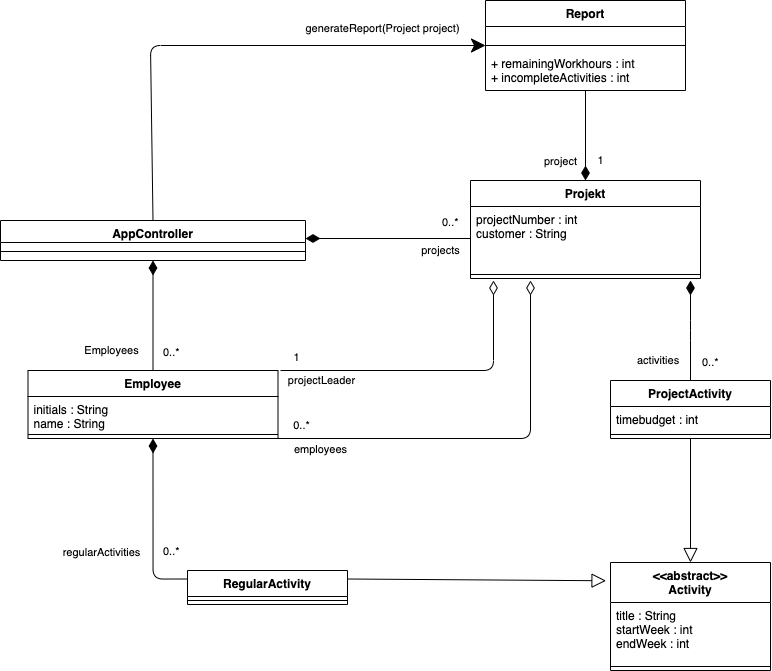
\includegraphics[width = .75\textwidth]{Diagrams/Klassediagram_eng.png}
    % \caption{DANSK udkast af Klassediagram}\label{fig:ClassDiag}
    % 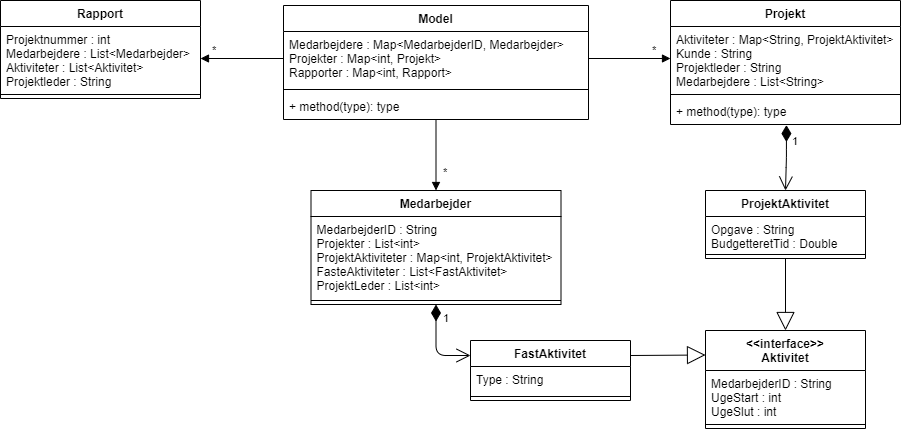
\includegraphics[width = .75\textwidth]{Diagrams/Klassediagram.png}
\end{figure}
\subsection{Sekvensdiagrammer}